\section{Eggstatic about the potential Below Zimmer}

\margininbox{Below Zimmer}{
     \begin{itemize}
    \item Jana Čarga
    \item James Kirkpatrick
    \item Dave Wilson
    \end{itemize}}{\explo}

James and Dave went for a quick bounce trip to look at the undescended
pitch below \passage{Zimmer} chamber, which started with a traverse in a
rift part-filled with boulders.

Bolts for the traverse led to a point where a drop into a water could be
seen. On bolting and descending this, the landing was in a shallow pool,
with water coming from some way back in the rift, having been collected
on the floor of \passage{Zimmer} chamber after running through the boulders
from both waterfalls.


\begin{pagefigure}
      \checkoddpage \ifoddpage \forcerectofloat \else \forceversofloat \fi
    \centering
    \begin{subfigure}{0.49\textwidth}
        \frame{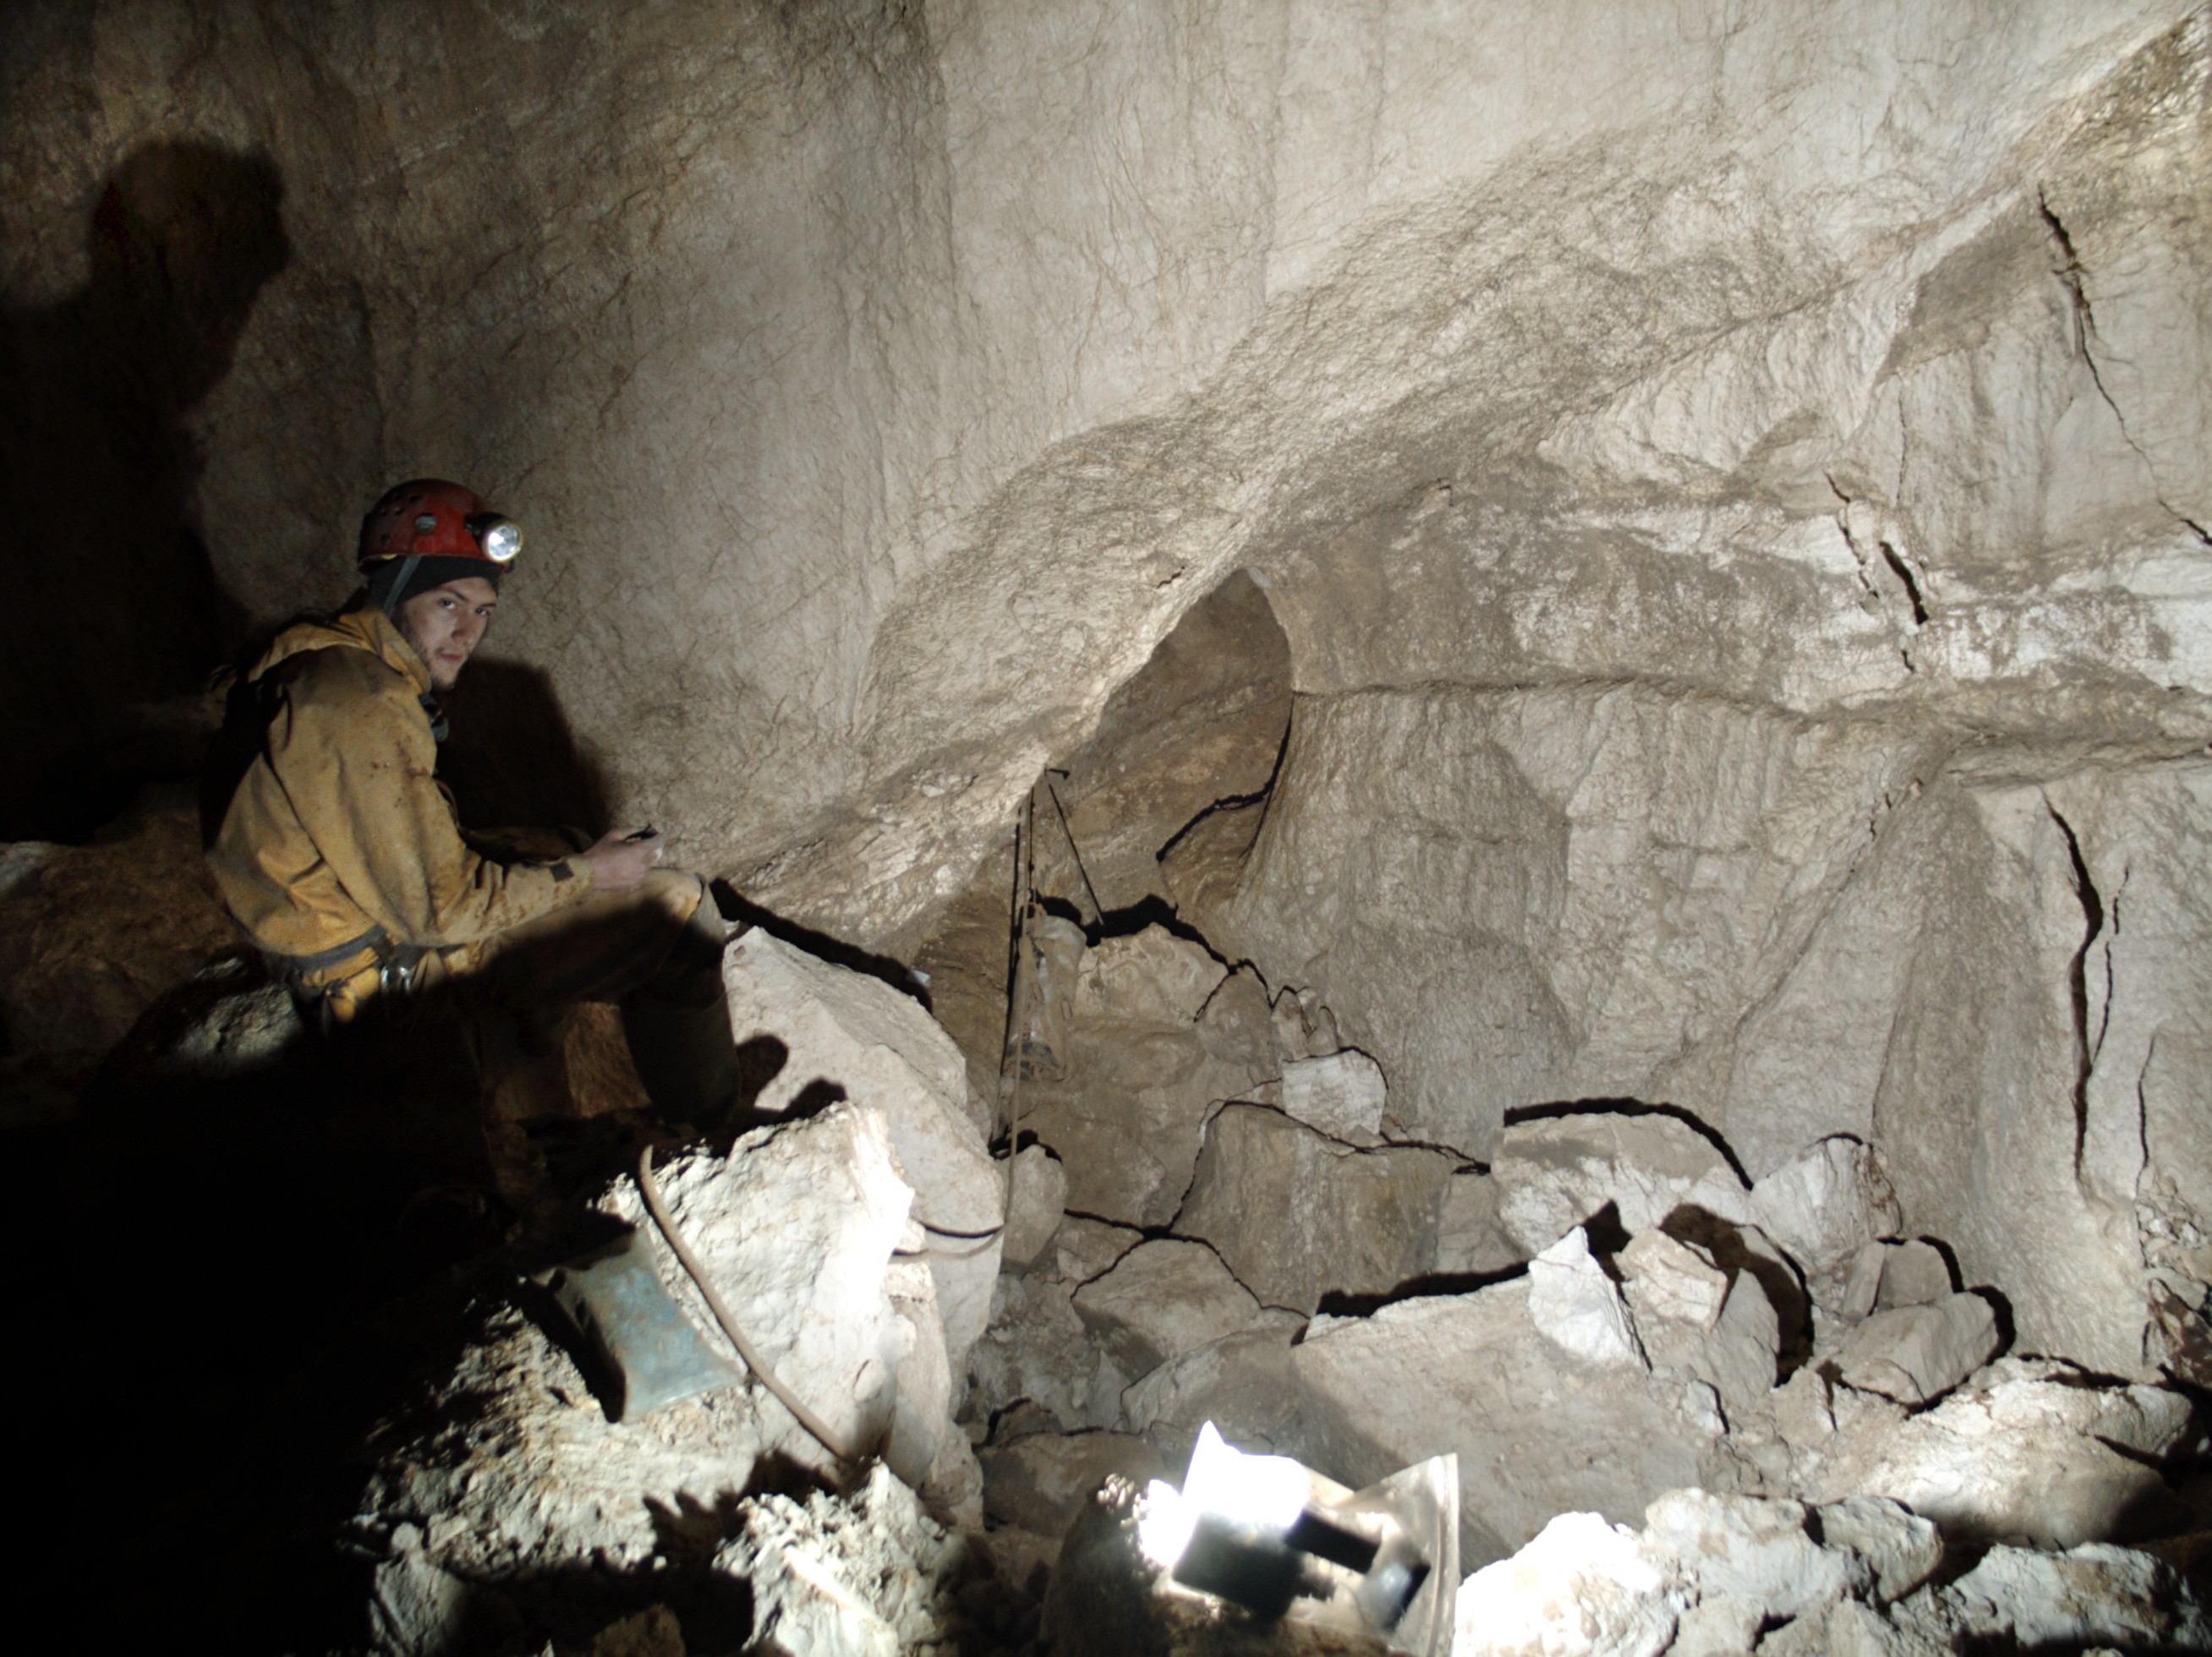
\includegraphics[width=\linewidth]{2009/zimmer/2009-08-16-15.35.20 - Jarvist Frost - Canon Powershot G5 - Zimmer entrance to Eggstacy--orig.jpg}} 
        \caption{} \label{below zimmer entry}
    \end{subfigure}
\hfill
    \begin{subfigure}{0.49\textwidth}
    \centering
        \frame{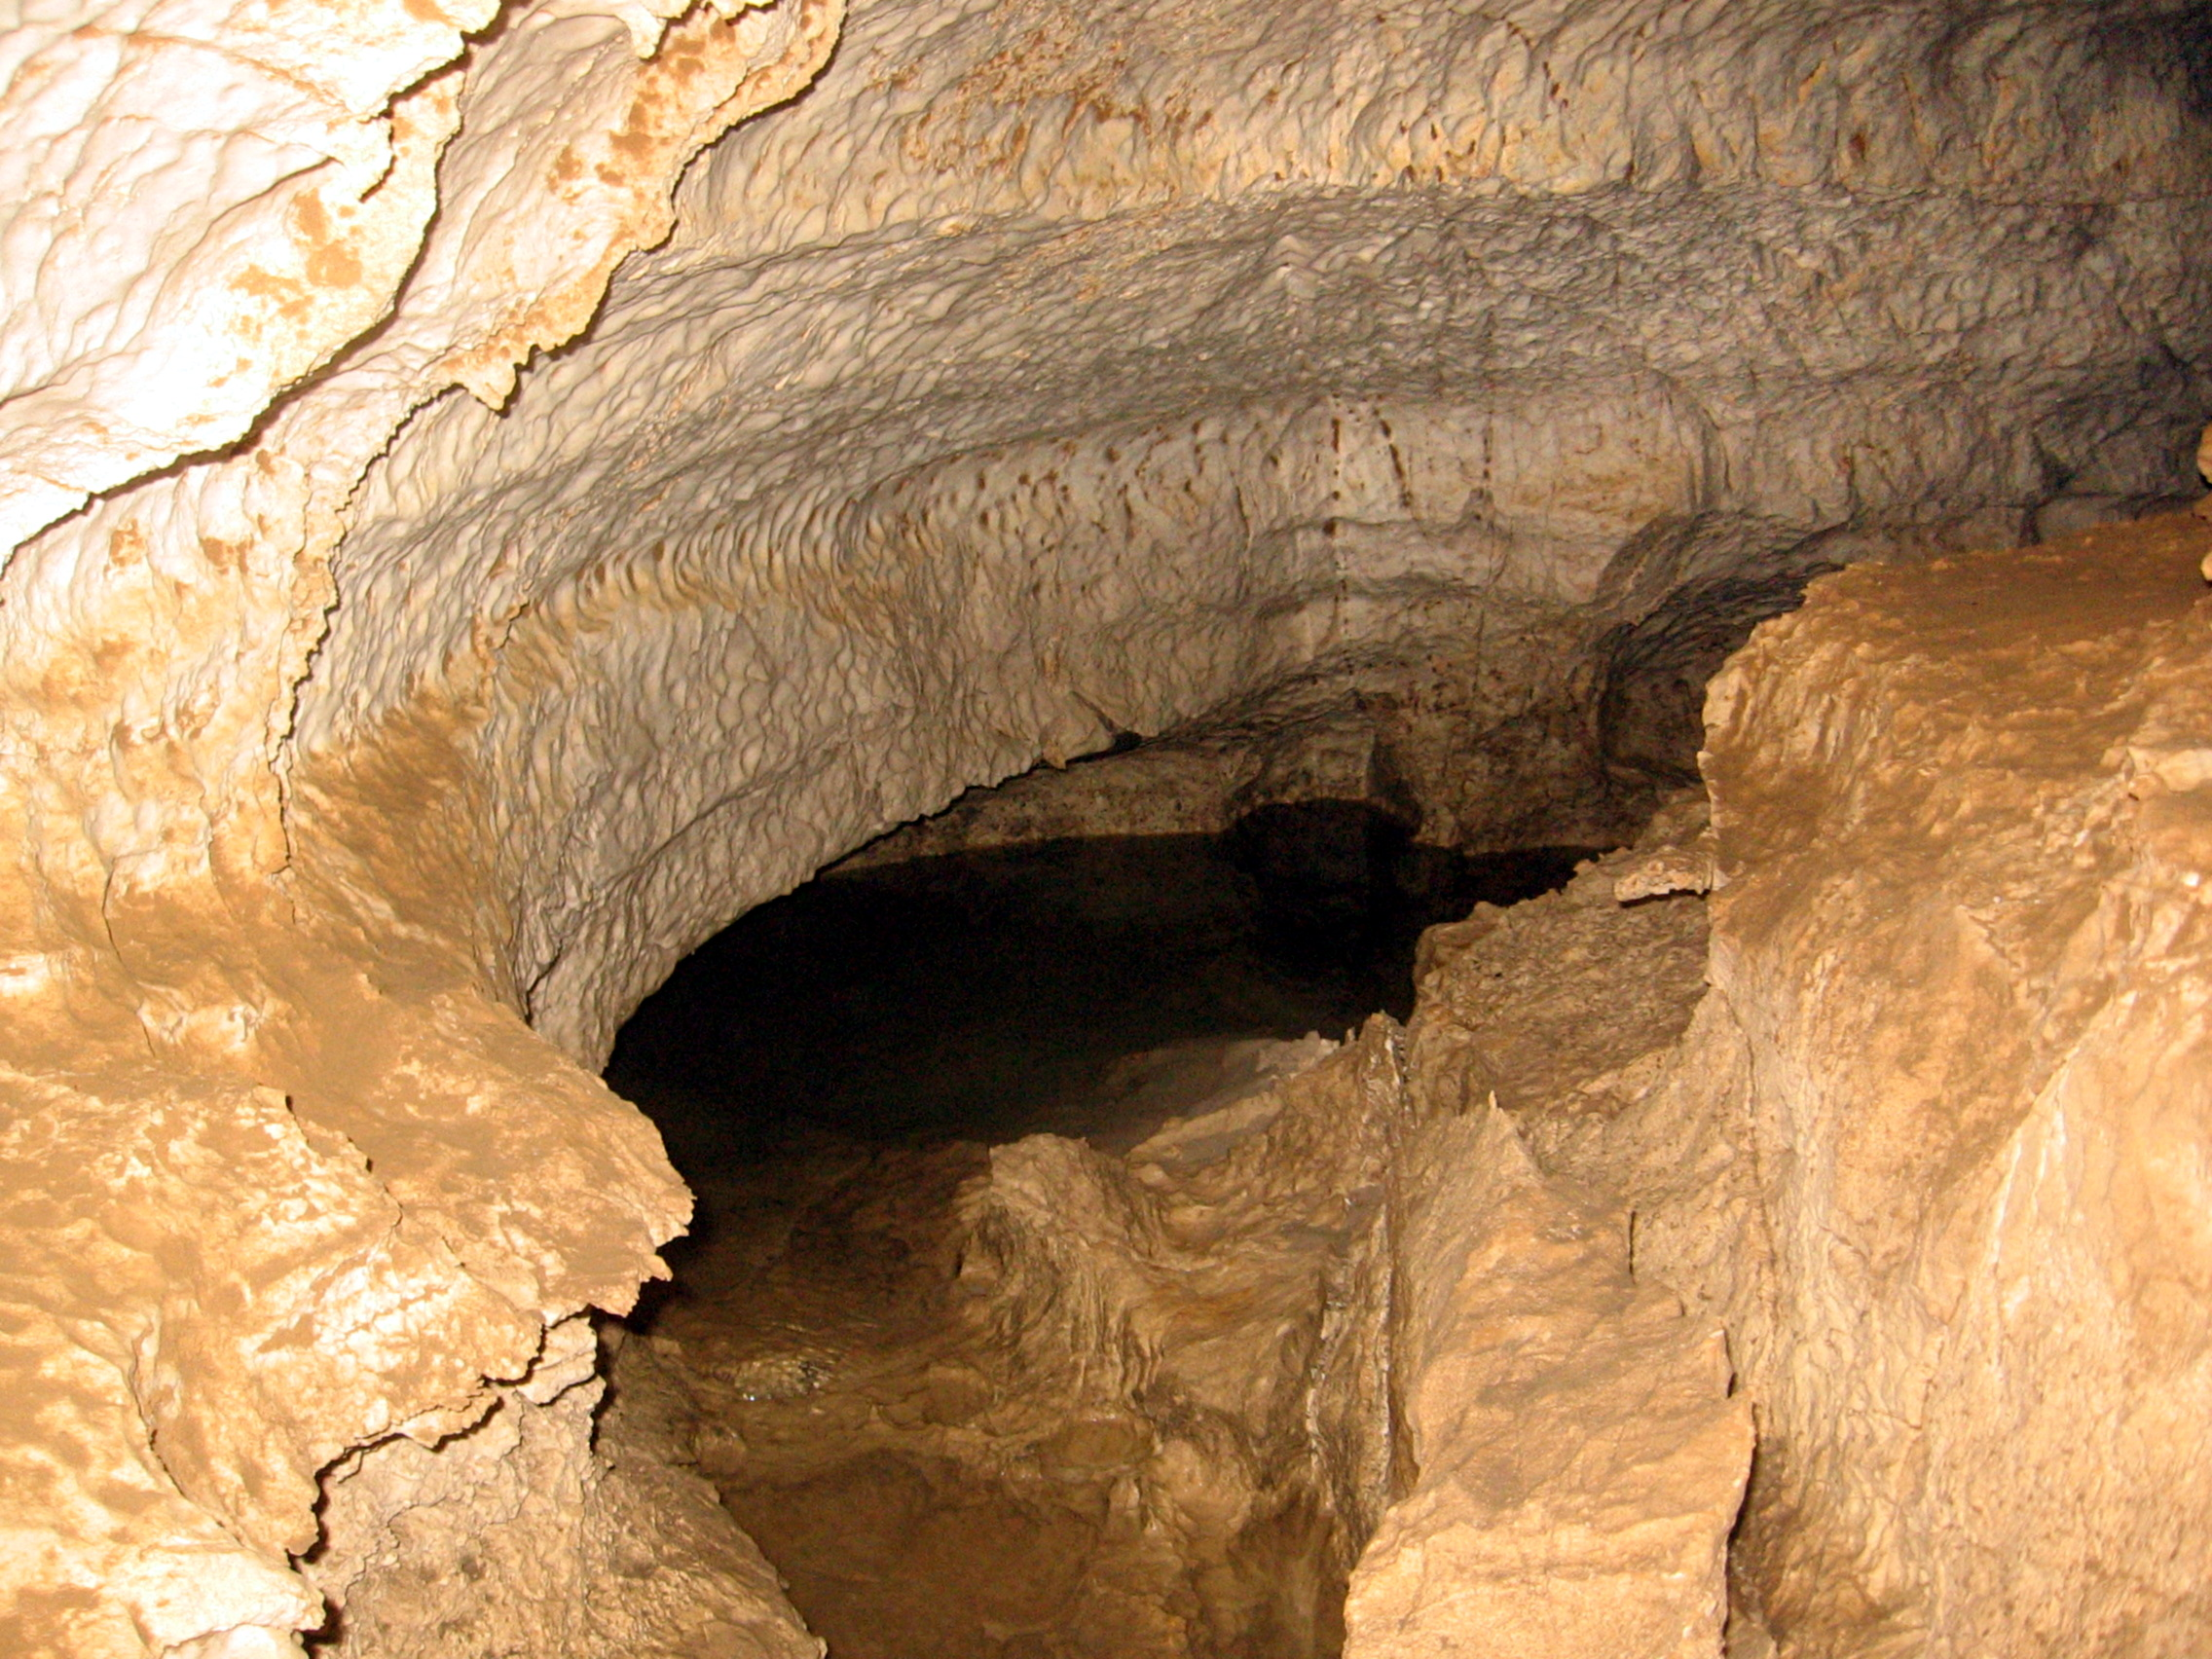
\includegraphics[width=\linewidth]{2009/zimmer/2009-08-15-21.35.42 - Jana Carga - Canon Powershot A520 - Cascade on way to first pitch below zimmer--orig.jpg}} 
        \caption{} \label{below zimmer cascade}
\end{subfigure}
\vfill
\begin{subfigure}{0.49\textwidth}
    \centering
        \frame{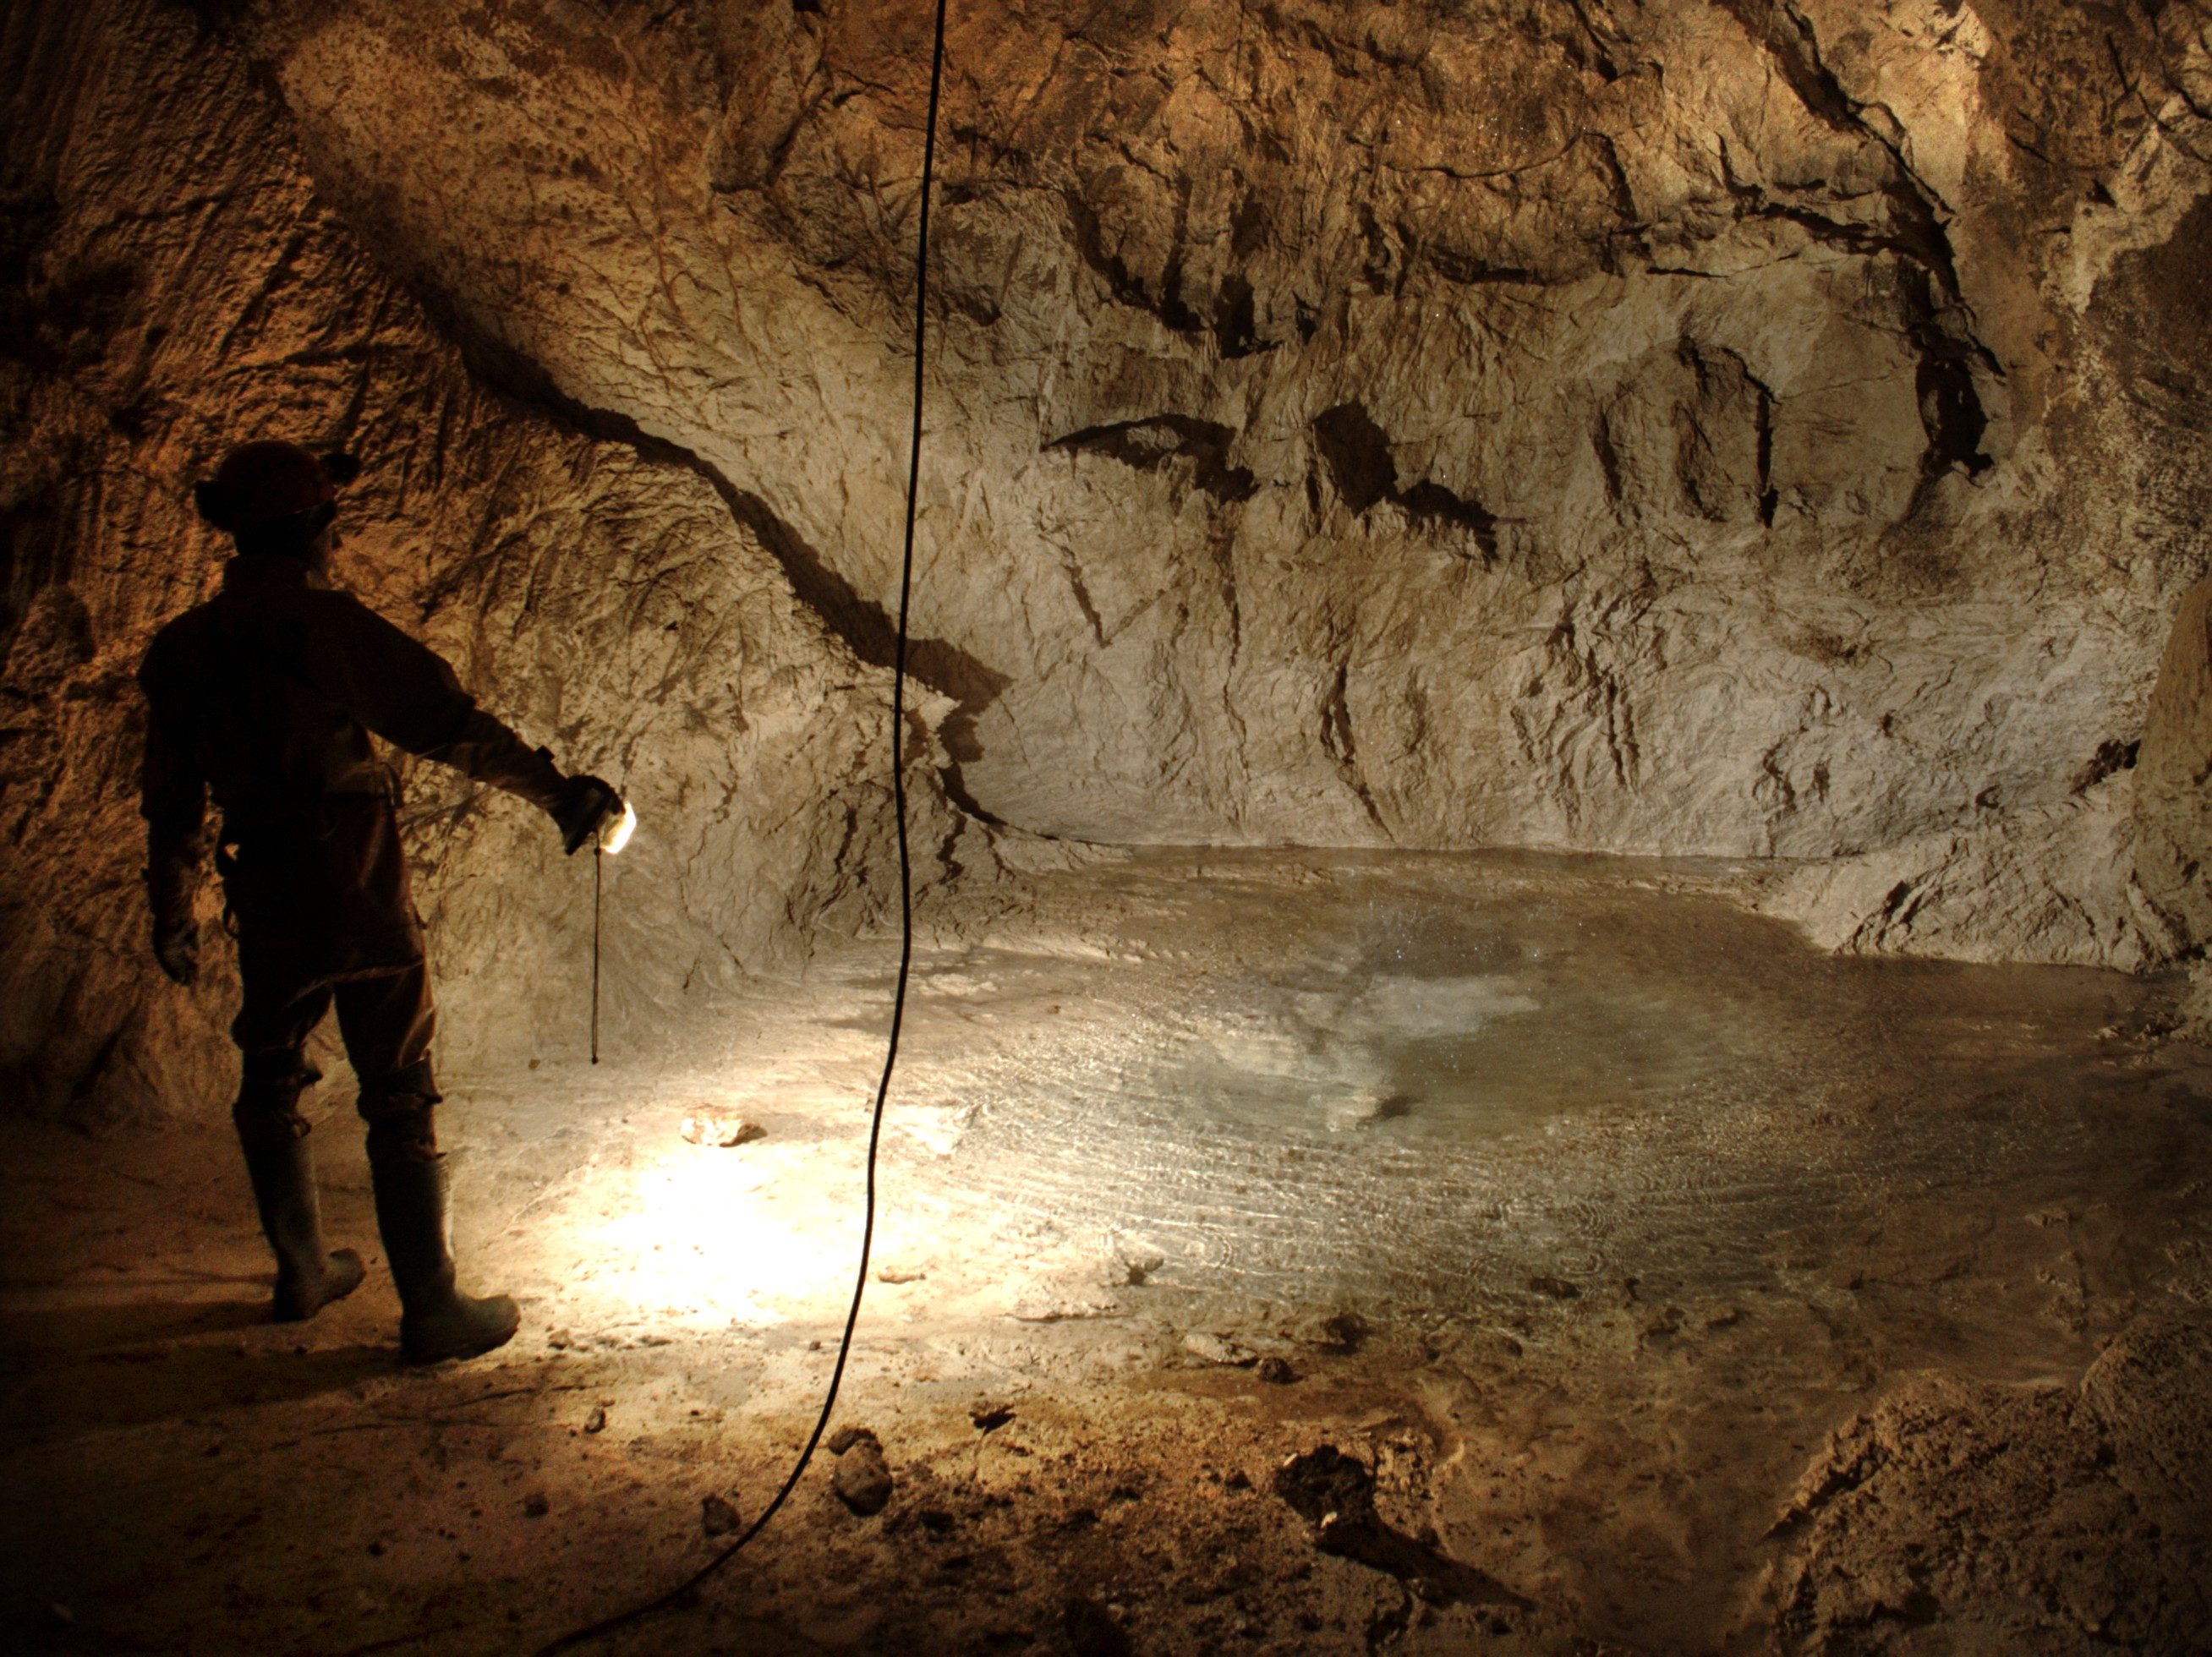
\includegraphics[width=\linewidth]{2009/zimmer/2009-08-16-15.03.00 - Jarvist Frost - Canon Powershot G5 - Eggstacy - below zimmer - first pitch--orig.jpg}} 
        \caption{} \label{below zimmer first pool}
\end{subfigure}
\hfill
\begin{subfigure}{0.49\textwidth}
    \centering
        \frame{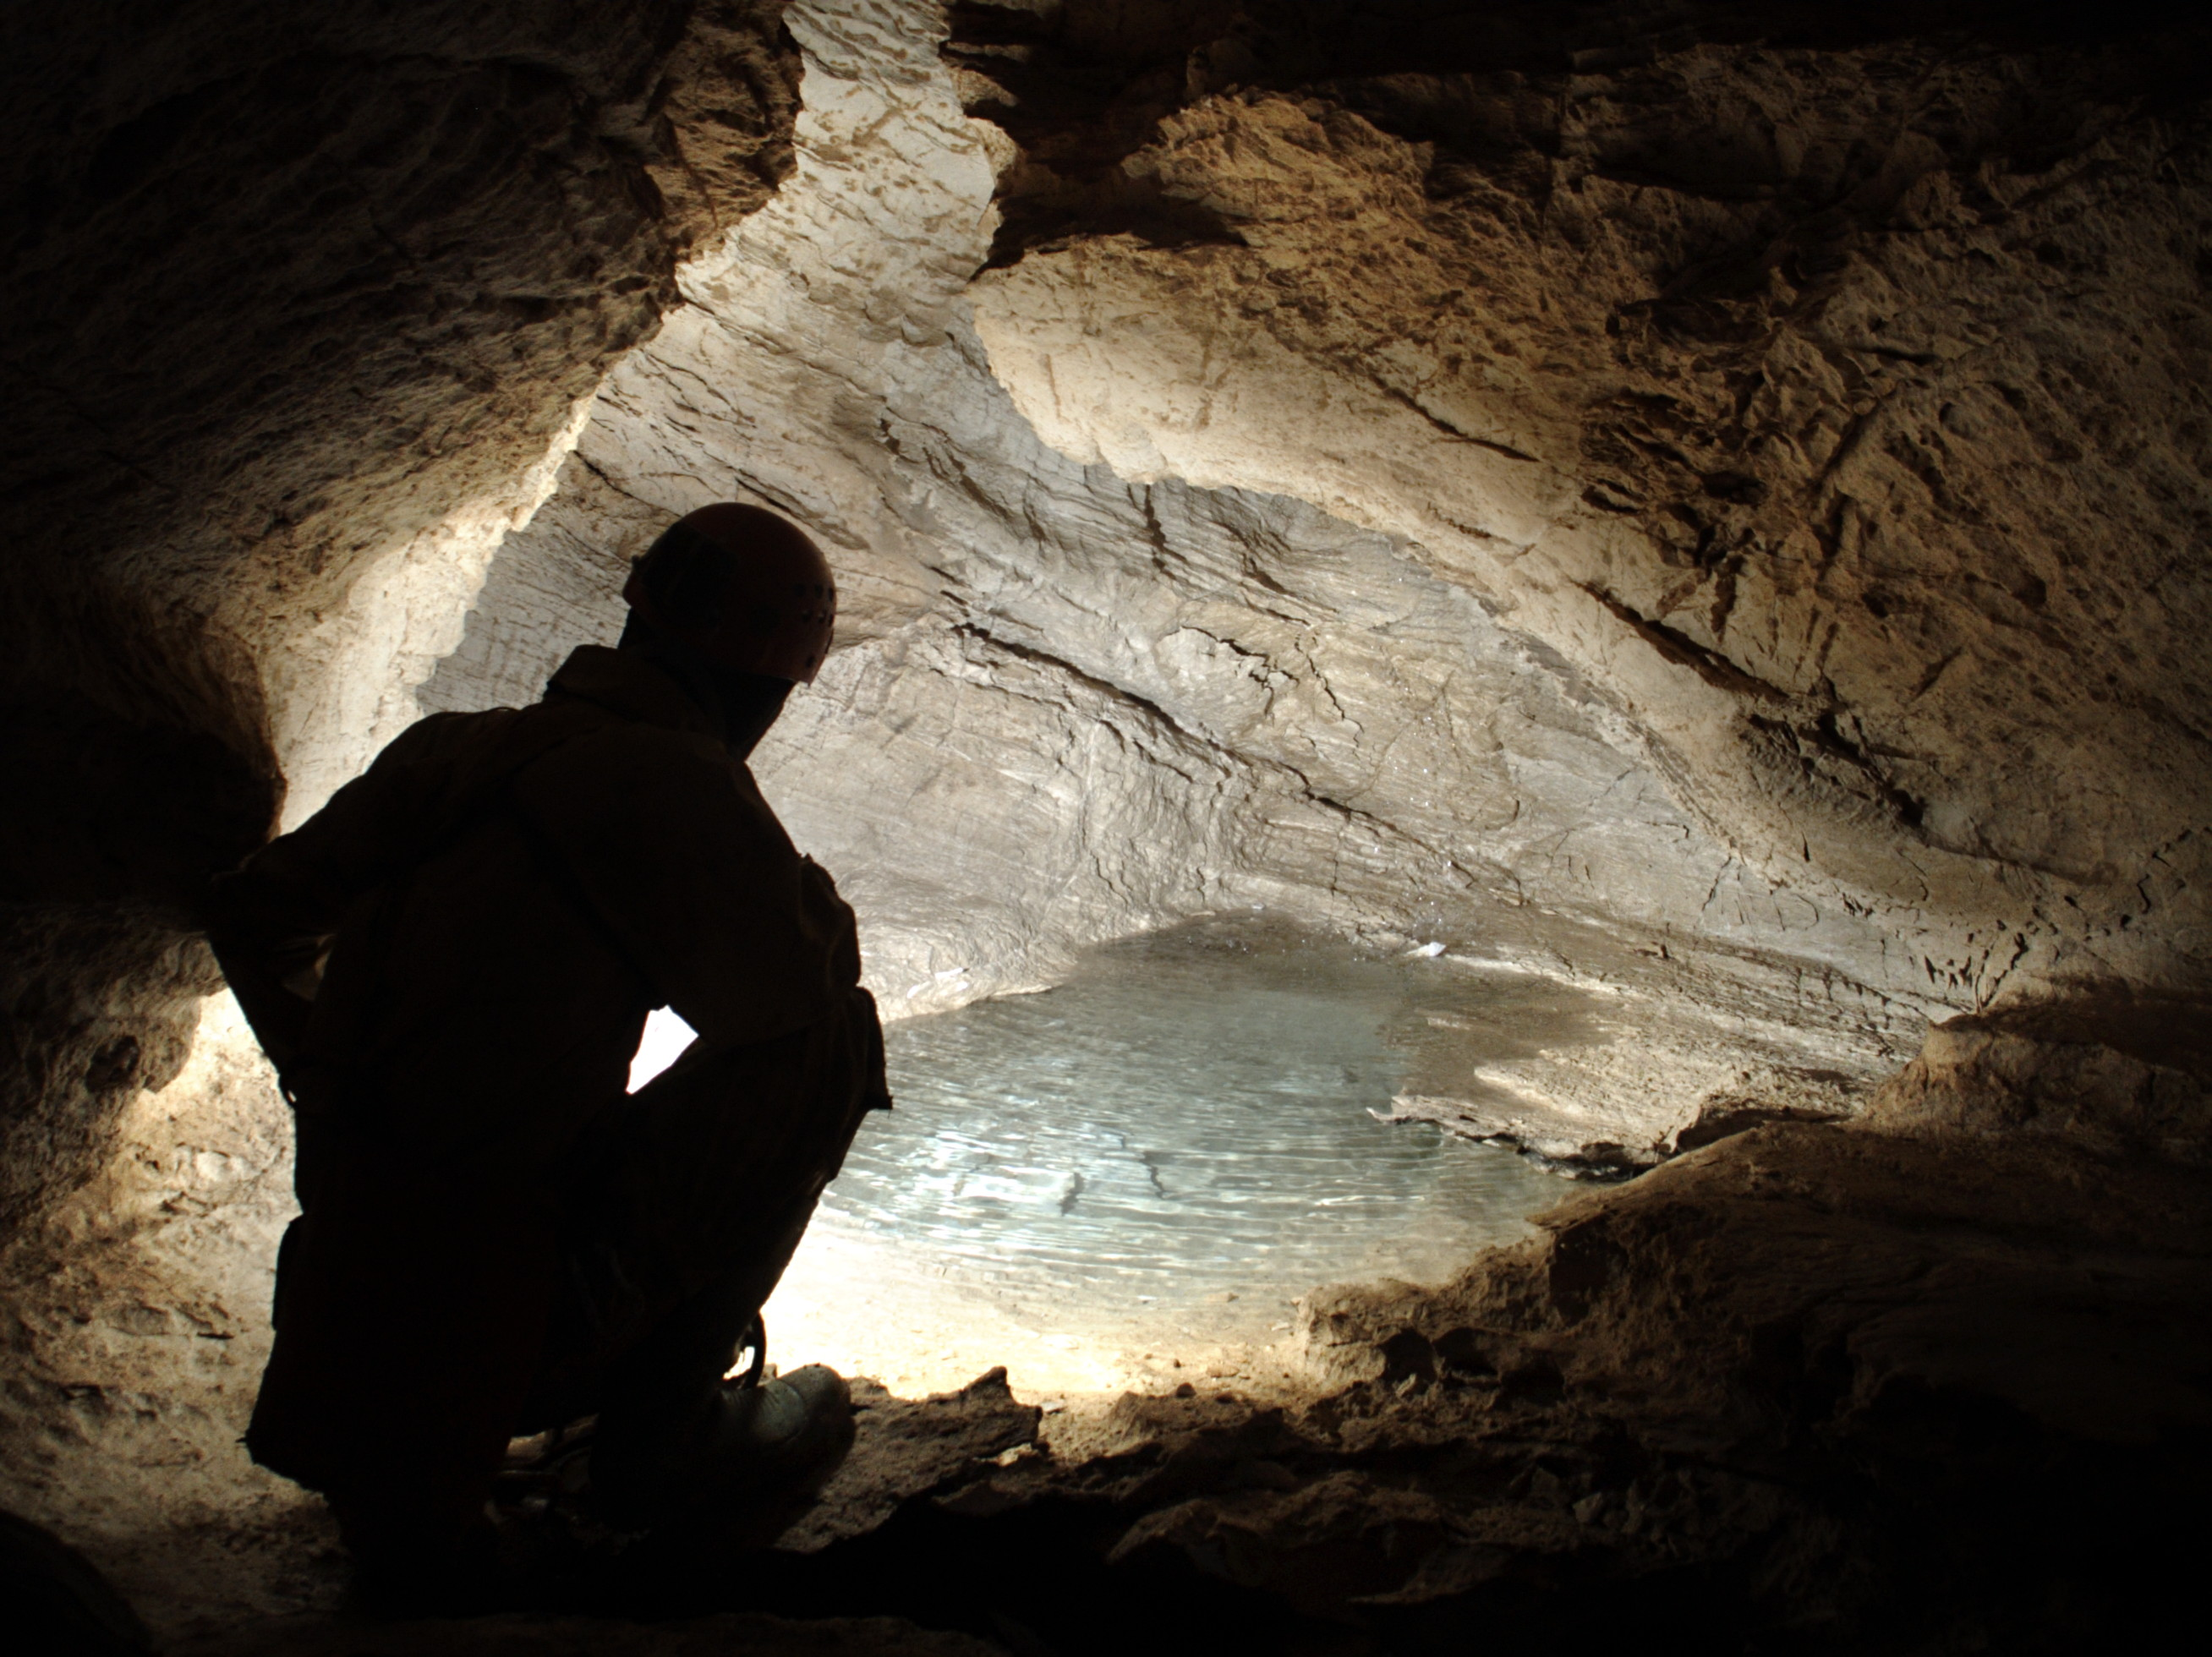
\includegraphics[width=\linewidth]{2009/zimmer/2009-08-16-15.09.58 - Jarvist Frost - Canon Powershot G5 - Eggstacy - below zimmer - 2nd plunge pool--orig.jpg}}
        \caption{} \label{below zimmer second pool}
    \end{subfigure}
 \caption{\protect\passage{Below Zimmer.} \textit{a)} The entrance to the area from \protect\passage{Zimmer}. \pic{Jarvist Frost} \textit{b)} Cascade on the way to the first pitch, Eggstravaganza, in \protect\passage{below Zimmer}. \pic{Jana Čarga} \textit{c)} First pool beneath the first pitch. \textit{d)} Second pool beneath the first pitch. \pic{Jarvist Frost} }
\end{pagefigure}


The water then ran from the pool to cascade down a series of short drops
in a clean-washed rift with a friable slabby roof/wall overhanging it,
and eventually a point was reached with a drop too long to free-climb
down, with the passage beyond bending to the left and seeming to carry
on descending.

This certainly seemed like it had some potential, and was interesting in
that (with the exception of \passage{Republika}) it was the first
decent-flow active streamway encountered at depth as part of a main
route, rather than a streamway crossing the passage appearing from and
going to nowhere accessible.

A pleasant little bounce trip with an interesting and attractive find.

\name{Dave Wilson}


James, Jana and Dave returned a couple of days later to push a little
and take photographs, and while James and Jana got to work, Dave went to
drop a rope down to \passage{Falls Road} from \passage{Friendship Gallery},
since the \passage{Capt. K.} crew had seemed likely to have reached there at a
lower level a day or two before, and a rope would enable a through-trip. On descending, their anchors were found, showing that they actually had
been where we had calculated.

\name{Dave Wilson}


\subsection{15-8-09 -- Down to \passage{Zimmer} and the connection}

 \margininbox{Falls Road}{
     \begin{itemize}
    \item Gergely Ambrus
    \item Jana Čarga
    \item Dave Wilson
    \end{itemize}}{\explo}

The two goals of this trip were to find the rope that Tim and Thara
rigged from \passage{Happy Monday} plus survey and rig the rift below
\passage{Zimmer}.

The connection is found at \passage{Falls Road}. Climbing
down at the rift of the connection of \passage{Falls road} and
\passage{Friendship Gallery} a \textasciitilde 10 m drop reaches a Y hang
to the top of \passage{Free Amalgamation}. The bottom of \passage{Happy Monday} is
about 40 m away.

Below \passage{Zimmer} an active streamway is found with
beautiful lakes and a high meander. Top muddy passage of meander is
passable, but a drop down to the waterfalls would be better. Probably
the largest active known streamway on the mountain at the moment, highly
probably it leads somewhere unknown. Nice falls and waterfalls. Super nice trip -- show-cave area!

\name{Jana Čarga}
    
\begin{figure*}
\checkoddpage \ifoddpage \forcerectofloat \else \forceversofloat \fi
\frame{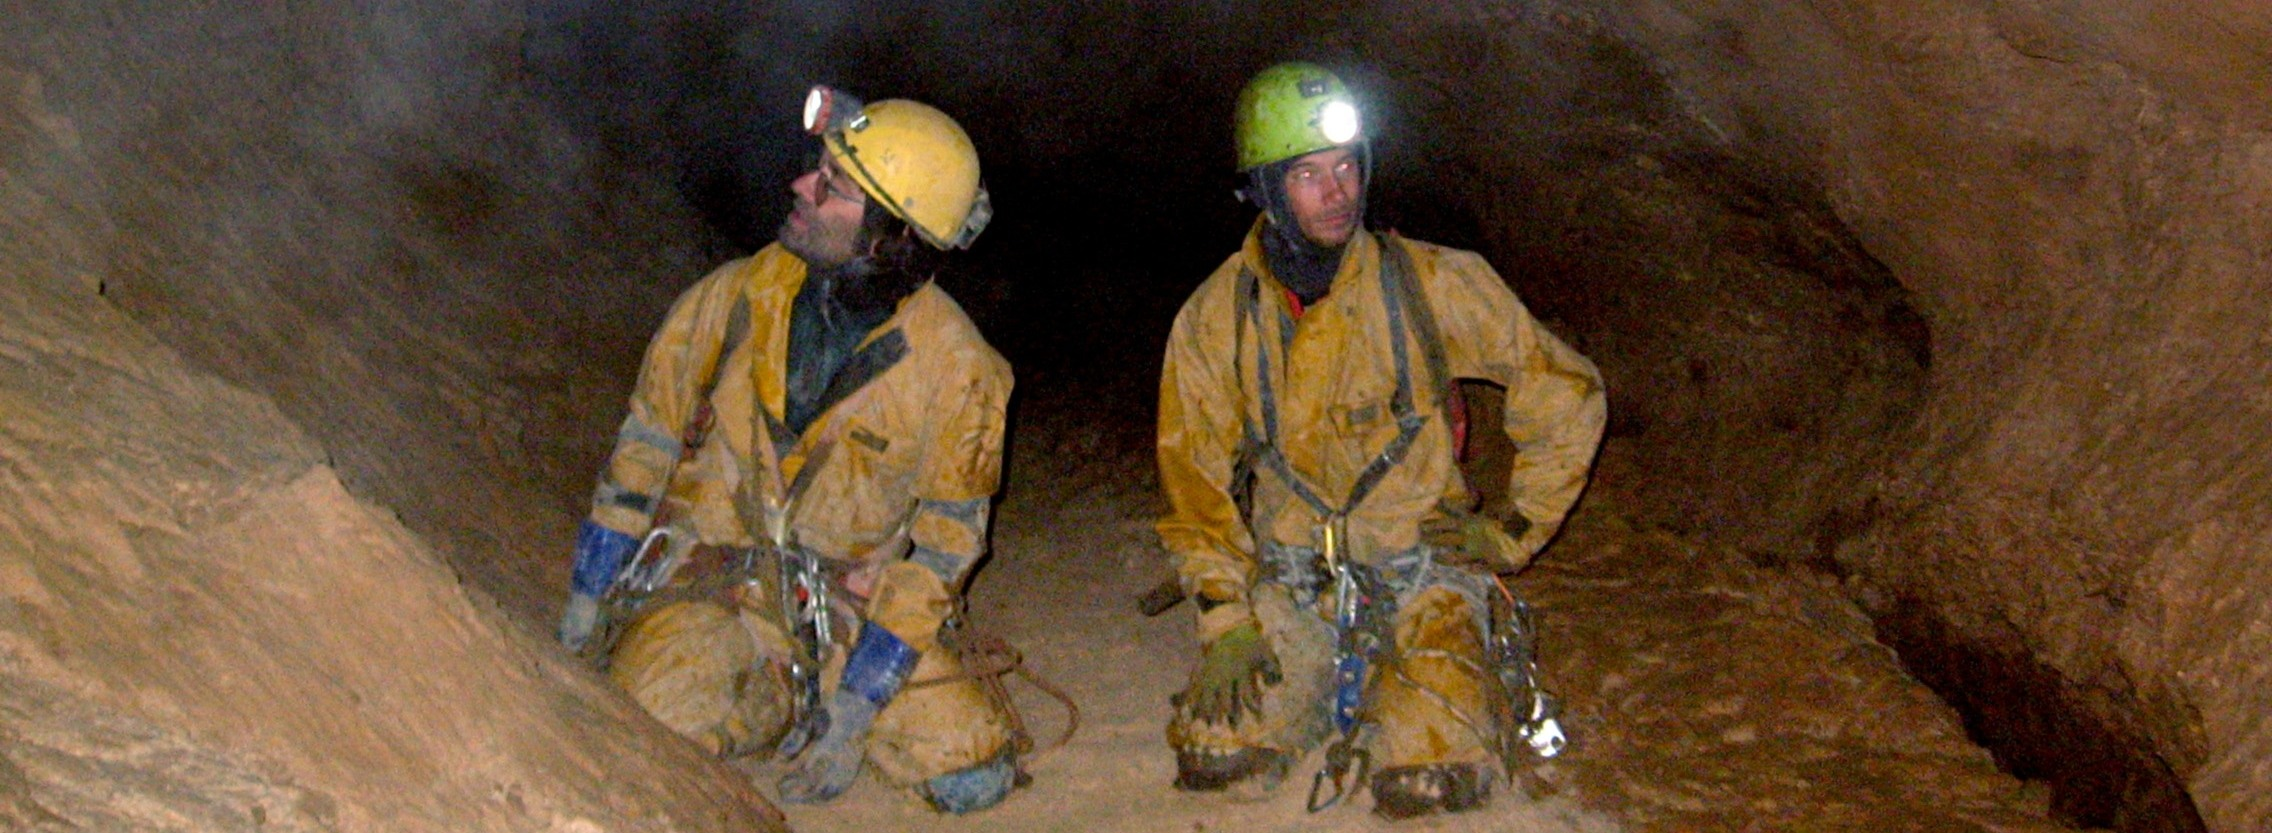
\includegraphics[width=\linewidth]{2009/zimmer/2009-08-15-19.14.16 - Jana Carga - Canon Powershot A520 - Friendship Gallery - Gergely and DaveW Flash--orig.jpg}}
\caption{Dave Wilson and Gergely Ambrus in \protect\passage{Friendship Gallery} on the way to \protect\passage{Falls Road}. \pic{Jana Čarga}}
\label{dave gergely friendship}
\end{figure*}
